\documentclass[../main.tex]{subfiles}
\graphicspath{{\subfix{../images/}}}
\begin{document}

  Para o desenvolvimento do projeto, foi criada uma metodologia própria composta por três etapas sequenciais: fundamentação, desenvolvimento e resultados e análises. A seguir, serão detalhadas cada uma dessas etapas.

  \subsection{Fundamentação}
  A primeira etapa teve como objetivo buscar referências para embasar o estudo dos robôs quadrúpedes e servir de padrão para o desenvolvimento do projeto.

  Primeiramente, foi realizada uma pesquisa bibliográfica com o intuito de selecionar artigos relacionados com o projeto. Para realizar essa busca, foi utilizado o método \textit{Bibliographic and Literary Review Method} (\textit{BiLi}), que consiste em um método de busca iterativa de artigos, guiada por análises estatísticas das palavras-chave e da rede de co-citação entre os trabalhos encontrados \cite{bili}.

  A partir dessa pesquisa, foi possível realizar um estudo do estado da arte com o objetivo de entender a teoria de locomoção dos robôs quadrúpedes. Além disso, foi feito um \textit{benchmarking} de projetos \textit{open source} desse tipo de sistema robótico, objetivando encontrar referências para a definição do conceito do robô que será projetado e, consequentemente, para a prototipação dele. Neste \textit{benchmarking}, foram buscados características que indicassem a viabilidade de prototipação, tais quais a disponibilidade do código na internet, a linguagem de programação utilizada, a disponibilidade do modelo 3D, se foi feito em impressão 3D ou não, o tipo dos atuadores e os sensores que foram utilizados.

  \subsection{Desenvolvimento}
  Durante esta etapa, houve o desenvolvimento do robô propriamente dito. Foram criadas duas frentes de trabalho que ocorreram em paralelo: a implementação e simulação dos algoritmos em ambiente computacional, e a criação do \textit{design} junto à prototipação do robô.

  Durante a implementação dos algoritmos na simulação, foram elaborados, primeiramente, o diagrama de blocos do sistema e a arquitetura de \textit{software} do controlador. A partir disso, os algoritmos de cinemática e controle foram implementados e testados na simulação. Para auxiliar o desenvolvimento do projeto, algumas ferramentas de \textit{softwares} foram utilizadas, como o \textit{ROS2 Humble} e o simulador \textit{Gazebo}.

  Em paralelo ao desenvolvimento do \textit{software}, foi realizado o \textit{design} e a prototipação do robô através da elaboração dos desenhos mecânicos e do projeto eletroeletrônico. Esta etapa incluiu também a impressão 3D das partes mecânicas, o teste dos atuadores e sensores e a configuração da comunicação entre a central de processamento e os atuadores, culminando na montagem física do protótipo. Durante essa etapa, o \textit{software} \textit{OnShape} foi utilizado para a modelagem 3D do robô e o \textit{QElectroTech}, para o projeto eletroeletrônico.

  Após essas duas etapas, foi possível realizar a integração dos algoritmos no protótipo físico. Ao final da integração, o protótipo já estava funcional e pronto para a fase de testes.

  \subsection{Resultados e análises}
  \label{sec:method_results_analysis}
  Durante a etapa de resultados e análises, foram feitos testes e experimentos a fim de avaliar a performance de locomoção do robô. Eles foram divididos em dois grupos: testes preliminares e experimentos de locomoção. Os testes preliminares objetivam testar duas funcionalidades básicas do robô: a movimentação do corpo com base no modelo cinemático e o controle de angulação do corpo. Esses testes são importantes porque ambas as funcionalidades são utilizadas nos experimentos de locomoção e influenciam diretamente no comportamento do robô.
  
  Foram realizados dois experimentos de locomoção com o objetivo avaliar a capacidade do robô de se locomover em terrenos planos e irregulares. O primeiro experimento consistiu em mover uma das patas por uma trajetória cicloidal feita pelo planejador de trajetórias. Para isso, o corpo do robô foi apoiado em um suporte elevado, de modo que as patas não tocassem o chão, diminuindo a carga sobre os motores. O objetivo principal deste teste foi verificar se o sistema de controle do robô era capaz de responder de forma coerente aos comandos enviados pelo planejador de marchas numa situação mais próxima da ideal (sem carga). As trajetórias foram calculadas considerando a altura de passo $0,05 m$, período de $0,5 s$ e uma resolução de $25$ pontos distribuídos de forma homogênea ($P_T = P_N = 1,0$). Foram feitos dois testes nesse experimento, variando as distâncias que a pata deve percorrer nas coordenadas $x$ e $y$. Para cada teste, foram coletadas 30 amostras.
  
  O segundo experimento teve como objetivos verificar a capacidade do robô de seguir um comando de velocidade pré-estabelecido e de manter a orientação do seu corpo estável em $0\degree$ nos ângulos de \textit{roll} e \textit{pitch}. O experimento foi realizado em dois tipos de terreno: um chão de cimento plano (\ref{fig:terreno_plano}) e um terreno irregular formado por pequenas pedras soltas (\ref{fig:terreno_irregular}). Este experimento consistiu em enviar um comando de velocidade constante para frente de $0,05 m/s$ e medir o tempo que o robô precisou para percorrer $1,5 m$. Assim, foi possível inferir a velocidade média e compará-la com o comando enviado. Além disso, a fim de avaliar a contribuição do controle de angulação do robô para sua estabilidade, metade dos experimentos foram realizados com esta funcionalidade ativa e a outra não. A estabilidade do robô foi mensurada por meio da oscilação máxima do corpo do robô nos ângulos de \textit{roll} e \textit{pitch}. A trajetória utilizada para o passo possui as mesmas especificações do primeiro experimento, exceto pelos parâmetros de disposição dos pontos, cujos valores adotados foram $P_T = 0,66$ e $P_N = 0,33$. Os experimentos foram organizados em quatro combinações de testes, variando o tipo do terreno e o uso, ou não, do controle de angulação. Para cada um dos 4 testes, foram coletadas 10 amostras.

  \begin{figure}[!htb]
    \centering
    \caption{Terrenos dos testes.}
    \begin{subfigure}[t]{0.24\textwidth}
      \centering
      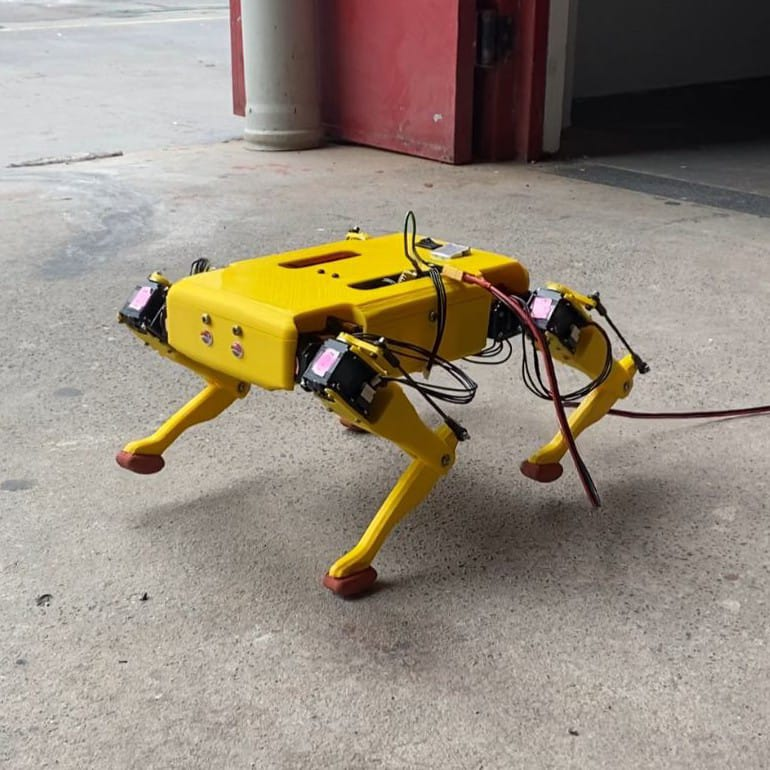
\includegraphics[width=1.0\textwidth]{terreno_plano.jpeg}
      \caption{Plano.}
      \label{fig:terreno_plano}
    \end{subfigure}
    \begin{subfigure}[t]{0.24\textwidth}
      \centering
      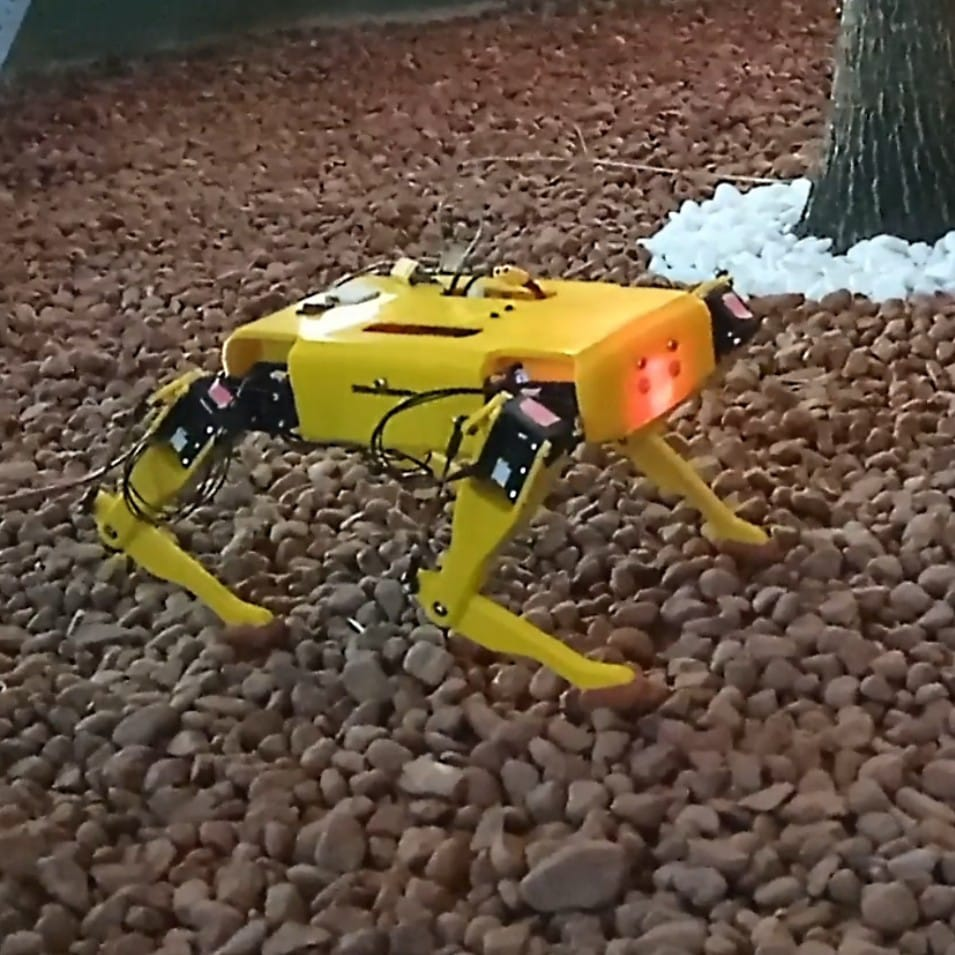
\includegraphics[width=1.0\textwidth]{terreno_irregular.jpeg}
      \caption{Irregular.}
      \label{fig:terreno_irregular}
    \end{subfigure}
    \vfill
    Fonte: autores.
    \label{fig:terrenos}
  \end{figure}
  
  % Por fim, foram feitos dois testes complementares a fim de checar a capacidade do robô de superar dois tipos de obstáculos: planos inclinados e degraus. Para o primeiro teste, foi construído um plano inclinado de aproximadamente $5,3\degree$ sobre o qual o robô deveria subir e descer. No segundo teste, foi testada a capacidade do robô de subir e descer degraus de 2, 4 e 5 centímetros. Ambos os testes foram feitos de forma teleoperada.

\end{document}
